\documentclass{article}
\usepackage[utf8]{inputenc}

\title{Assessment2-Performance}
\date{November 2020}

\usepackage{natbib}
\usepackage{graphicx}
\usepackage{minted}
\usepackage{pgfplots}

\begin{document}
\maketitle
\tableofcontents
\section{Introduction}

In this report, we design and carry out a performance experiment to investigate the behaviour or performance of the program, which solves the \emph{Percolate} problem in C code, when configured with different sized maps of the grid of squares. This report analyzes the performance of the program on seven different sizes of maps. The performance analysis includes the memory overhead and CPU overhead when the entire program is running. We also analyze the performance of the core code running time and the number of loops.

The remainder of this report is organized as follows: In Section 2, we designed a suitable method to analyze the performance of the memory overhead and CPU overhead respectively when running the entire program in the first two subsections. In the next two subsections, we analyze the performance of the running time and the number of loops respectively when running on the core code. In Section 3, we give the results of the above four experiments. In Section 4, we analyze and discuss the results. In Section 5, we summarize our work and give some suggestions for the future work. 

\section{Method}

We selected five sizes of maps for the experiment, the widths/heights are 20, 40, 80, 160, 320, 640 and 1280 respectively with a multiple of 2, while other parameters are default values. We didn't test the larger size because it is a time consuming work. Our program is compiled in \emph{gcc -g -c arralloc.c uni.c percolate.c $\mid$ gcc -g -o percolate arralloc.o uni.o percolate.o -lm $\mid$ ./percolate} with \emph{gcc 9.3.0} in \emph{Ubuntu 10.04.1}, \emph{Intel Core i5-9400F(one core)}, \emph{4G RAM}. We run program three times for each size of an experiment and take the average of the results.

\subsection{Memory Overhead}
We use Valgrind, a free memory debugging tool for Linux, to get the memory overhead of the entire program at runtime. We use command \emph{sudo apt-get install -y valgrind} in Ubuntu to install it. We use command \emph{valgrind ./percolate} to get the memory overhead, also we can add flag \emph{--leak-check=yes} to check whether there exists one(more) memory leak(s).

\subsection{CPU Overhead}
We use \emph{top} command to monitor CPU resource usage on Linux. It shows resource usage of all processes while we just need to show usage of our program, thus we use \emph{grep}  command to filter the result. The default refresh time interval is 3 seconds and we can use \emph{-d} flag to set it. The final command we use to get the CPU overhead is \emph{top -d 0.00001 $\mid$ grep percolate} and we run our program in another console terminal.

\subsection{Running Time}
We use a simple method to analyze the running time and number of loops experiments that we modify the program to analyze the running time of the core code as shown in Figure \ref{figure:code}. 

We use \emph{clock()} function and \emph{CLOCKS\_PER\_SEC} in \emph{time.h} to get the running time in seconds of the core code. We also comment the \emph{printf()} function to eliminate the influence of console output. 

We can also use \emph{gprof}, a profiling program which can collect timing information during program running. We install it by command \emph{sudo apt-get install binutils}, then we run \emph{gprof} we get \emph{a.out: No such file or directory} which means it installed successful. When we compile our program, we add flag \emph{-pg}, this means we will use \emph{gprof} to analyze it. We run our program and get a file named \emph{gmon.out}, that we can not read it directly so we convert it into information we can read by \emph{gprof percolate gmon.out $\textgreater$ out.txt}. We can get running time of all of the functions as shown in Figure \ref{figure:gprof}. We encapsulate the core code into a function to get more accurate running time result.

\begin{figure}[H]
  \centering
  \centerline{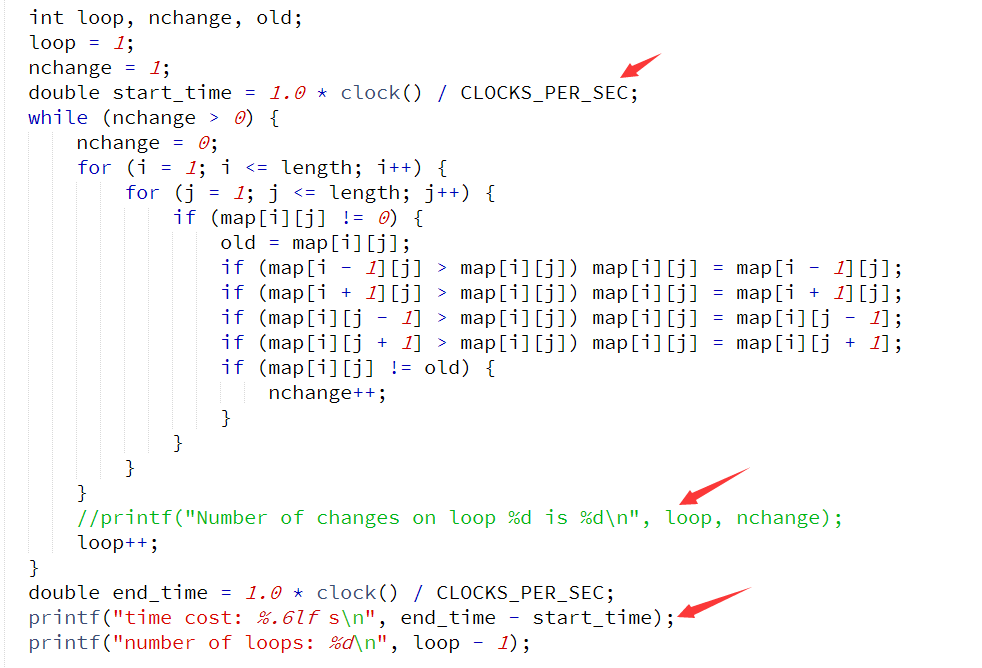
\includegraphics[width=300pt]{1.png}}
  \caption{Modified Core Code.}
\label{figure:code}
\end{figure}

\begin{figure}[H]
  \centering
  \centerline{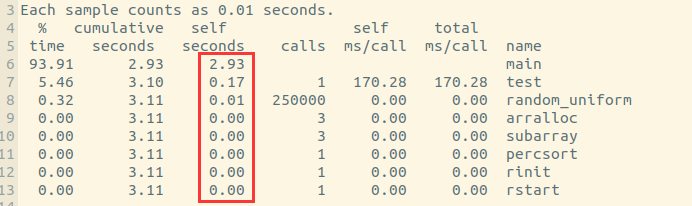
\includegraphics[width=300pt]{3.png}}
  \caption{Gprof Profiling Result.}
\label{figure:gprof}
\end{figure}

\subsection{Number of Loops}

As the description in Section 2.3, we get the results of running time and number of loops simultaneously.

\section{Results}
\subsection{Memory Overhead}
The result of the data that we get from experiment is shown in Table \ref{table:memory overhead} and Figure \ref{figure:memory overhead}.

\begin{table}[H]
\scriptsize
\centering
\label{table:memory overhead}
\begin{tabular}{c|c}%center or left or right
\hline\noalign{\smallskip}
Map Size & Memory Overhead(bytes)\\
\noalign{\smallskip}\hline\noalign{\smallskip}
20 & \textbf{20,304}\\
40 & \textbf{49,584}\\
80 & \textbf{165,744}\\
160 & \textbf{628,464}\\
320 & \textbf{2,475,504}\\
640 & \textbf{9,855,984}\\
1280 & \textbf{39,362,544}\\
\noalign{\smallskip}\hline
\end{tabular}
\caption{Memory Overhead.}
\end{table}

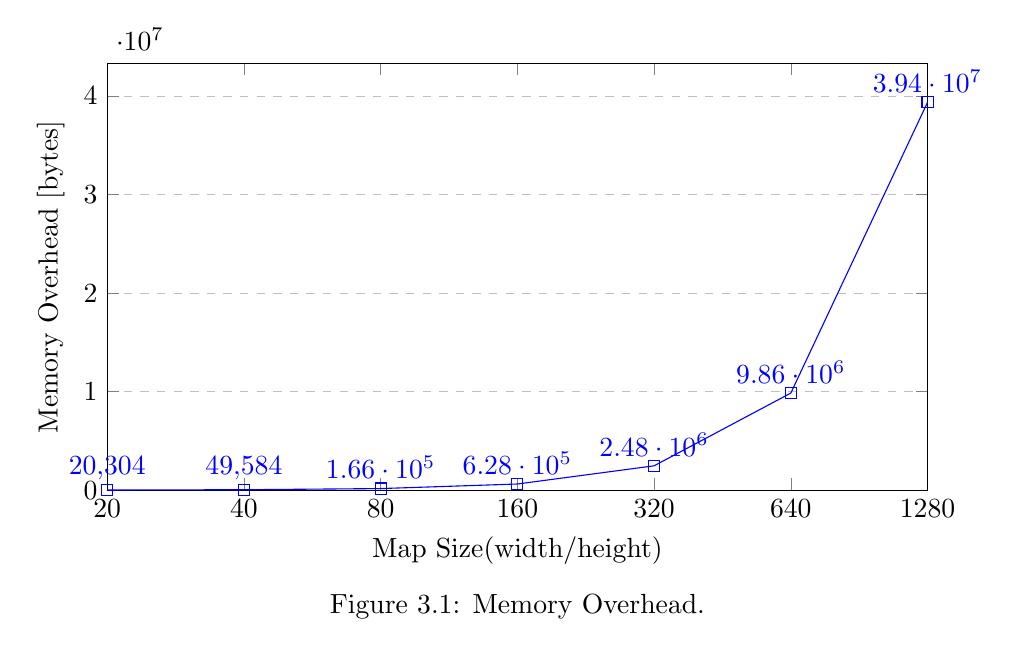
\begin{tikzpicture}
\label{figure:memory overhead}
\begin{axis}[
    width=12cm,height=7cm,
    nodes near coords,%show data.
    title style={at={(0.5,0)},anchor=north,yshift=-40},
    title={Figure 3.1: Memory Overhead.},
    xlabel={Map Size(width/height)},
    ylabel={Memory Overhead [bytes]},
    xmin=20, xmax=1280,
    ymin=0,
    symbolic x coords={20,40,80,160,320,640,1280},
    xtick=data,
    % ytick={1e1,1e2,1e3,1e4,1e5,1e6,1e7,1e8},
    legend pos=north west,
    ymajorgrids=true,
    grid style=dashed,
]

\addplot[
    color=blue,
    mark=square,
    ]
    coordinates {
    (20,20304)(40,49584)(80,165744)(160,628464)(320,2475504)(640,9855984)(1280,39362544)
    };

\end{axis}
\end{tikzpicture}

\subsection{CPU Overhead}
We find out that \emph{top} command can not capture the CPU usage if the program run too fast, e.g., map size is 20,40,80. We also find out that program use almost entire CPU resource in all cases, led to result of 99.9\% CPU usage as shown in Figure \ref{figure:cpu overhead} with red frame. 

\begin{figure}[H]
  \centering
  \centerline{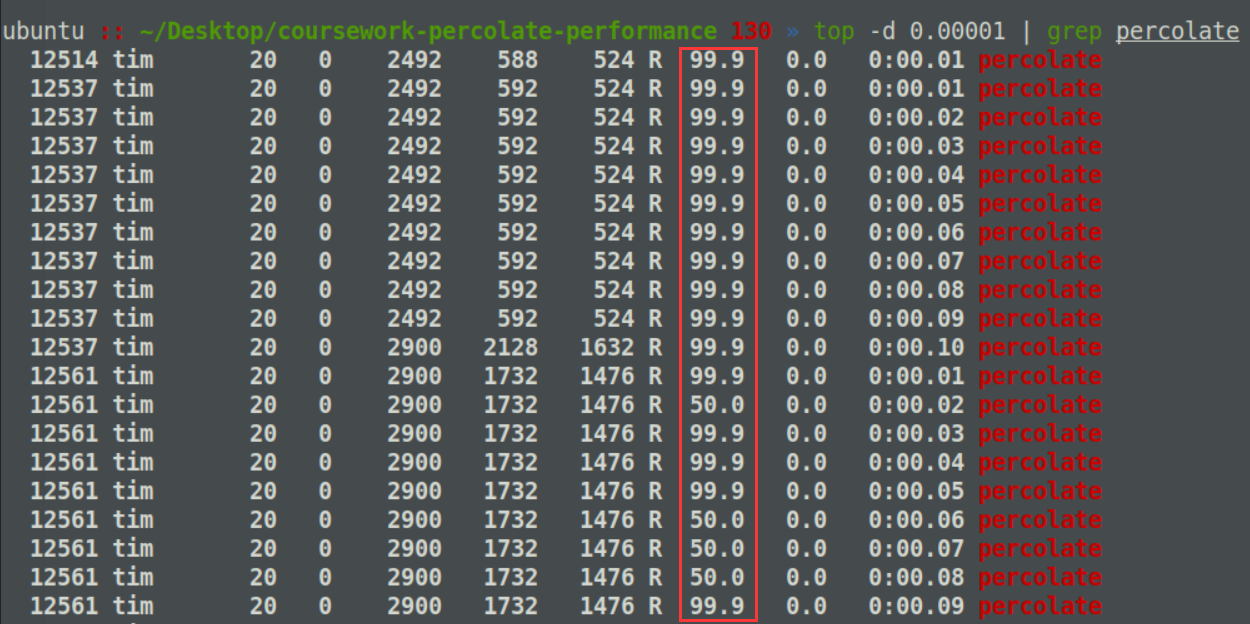
\includegraphics[width=300pt]{2.png}}
  \caption{CPU Overhead.}
\label{figure:cpu overhead}
\end{figure}

\subsection{Running Time}
The result of the data that we get from experiment is shown in Table \ref{table:running time} and Figure \ref{figure:running time}.

\begin{table}[H]
\scriptsize
\centering
\label{table:running time}
\begin{tabular}{c|ccc|c}%center or left or right
\hline\noalign{\smallskip}
Map Size & 1st Running & 2nd Running & 3rd Running & Average\\
\noalign{\smallskip}\hline\noalign{\smallskip}
20 & 0.000105 & 0.000104 & 0.000104 & \textbf{0.000104}\\
40 & 0.001237 & 0.001255 & 0.001248 & \textbf{0.001247}\\
80 & 0.011151 & 0.011267 & 0.011818 & \textbf{0.011412}\\
160 & 0.100917 & 0.095535 & 0.095107 & \textbf{0.097186}\\
320 & 0.759420 & 0.762362 & 0.756712 & \textbf{0.759498}\\
640 & 6.120218 & 6.118672 & 6.146592 & \textbf{6.128490}\\
1280 & 48.646746 & 48.865194 & 48.928090 & \textbf{48.813300}\\
\noalign{\smallskip}\hline
\end{tabular}
\caption{Running Time Result in Second.}
\end{table}

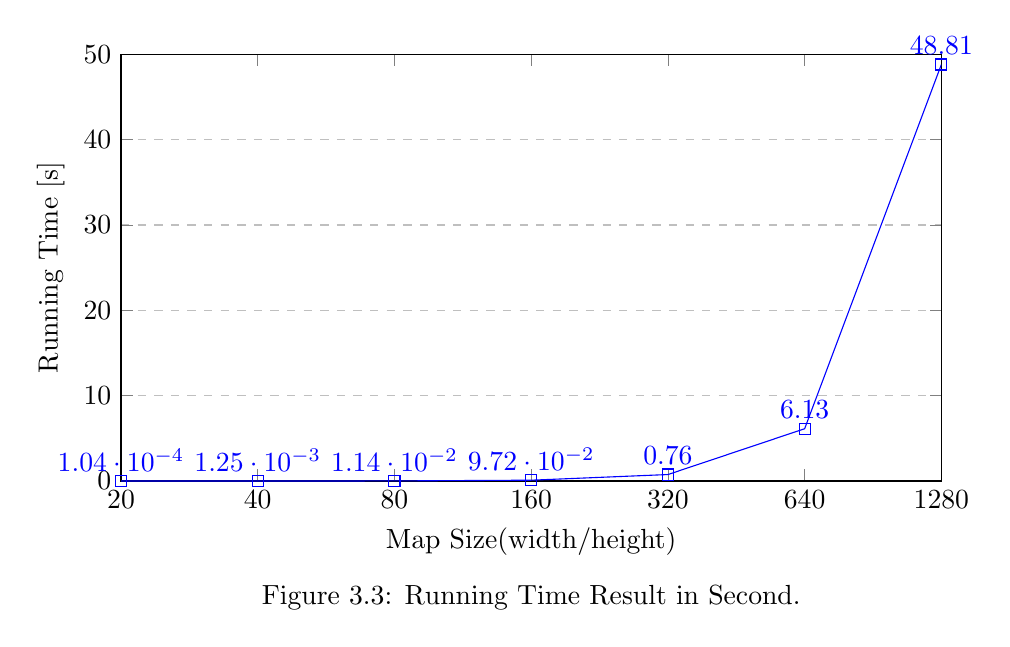
\begin{tikzpicture}
\label{figure:running time}
\begin{axis}[
    nodes near coords,%show data.
    width=12cm,height=7cm,
    title style={at={(0.5,0)},anchor=north,yshift=-40},
    title={Figure 3.3: Running Time Result in Second.},
    xlabel={Map Size(width/height)},
    ylabel={Running Time [s]},
    xmin=20, xmax=1280,
    ymin=0, ymax=50,
    symbolic x coords={20,40,80,160,320,640,1280},
    xtick=data,
    ytick={0,10,20,30,40,50},
    legend pos=north west,
    ymajorgrids=true,
    grid style=dashed,
]

\addplot[
    color=blue,
    mark=square,
    ]
    coordinates {
    (20,0.000104)(40,0.001247)(80,0.011412)(160,0.097186)(320,0.759498)(640,6.128490)(1280,48.813300)
    };

\end{axis}
\end{tikzpicture}

\subsection{Number of Loops}
The result of the data we get from experiment is shown in Table \ref{table:number of loops} and Figure \ref{figure:number of loops}.

\begin{table}[H]
\scriptsize
\centering
\label{table:number of loops}
\begin{tabular}{c|c}%center or left or right
\hline\noalign{\smallskip}
Map Size & Number of Loops\\
\noalign{\smallskip}\hline\noalign{\smallskip}
20 & \textbf{28}\\
40 & \textbf{77}\\
80 & \textbf{159}\\
160 & \textbf{313}\\
320 & \textbf{633}\\
640 & \textbf{1284}\\
1280 & \textbf{2554}\\
\noalign{\smallskip}\hline
\end{tabular}
\caption{Number of Loops.}
\end{table}

{\centering
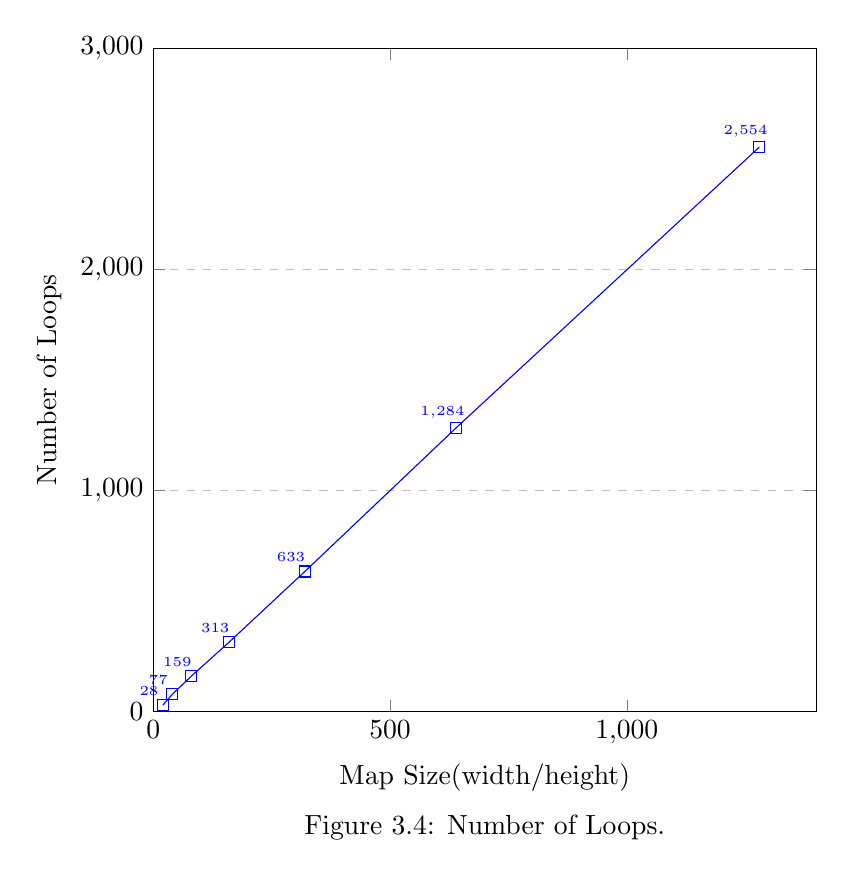
\begin{tikzpicture}
\label{figure:number of loops}
\begin{axis}[
    nodes near coords,%show data.
    every node near coord/.append style={xshift=-5pt,font=\tiny},
    width=10cm,height=10cm,
    title style={at={(0.5,0)},anchor=north,yshift=-40},
    title={Figure 3.4: Number of Loops.},
    xlabel={Map Size(width/height)},
    ylabel={Number of Loops},
    xmin=0, xmax=1400,
    ymin=0, ymax=3000,
    xtick={0,500,1000,1500},
    ytick={0,1000,2000,3000},
    legend pos=north west,
    ymajorgrids=true,
    grid style=dashed,
]

\addplot[
    color=blue,
    mark=square,
    ]
    coordinates {
    (20,28)(40,77)(80,159)(160,313)(320,633)(640,1284)(1280,2554)
    };

\end{axis}
\end{tikzpicture}
}


\section{Discussion}
All of our experiments show detailed data show in tables and figures in section 3 except monitoring in CPU overhead. This is because our computer allocates almost all CPU resources to run the program.

We can analyze from results of Figure \ref{figure:memory overhead} and \ref{figure:running time} in memory overhead and running time that the curves of both have similar shapes. This shows that there is a close coupling between memory overhead and running time, because the size of the map is directly related to the size of the memory used and the number of \emph{FOR} loop traversals. The larger the map size, the larger the memory required, and the more loops.

We can analyze from Figure \ref{figure:number of loops} that the map size and number of loops have a proportional relationship. Assume map size be $x$ and number of loops be $f$, then the relationship between them is $f\approx 2x$.

We once again analyze the result of running time only for the reason that running time and memory overhead have a close coupling. We divide one result by the previous result to get the ratio between two adjacent running time and the results are in Table \ref{table:ratio} and Figure 4.1.

\begin{table}[H]
\scriptsize
\centering
\label{table:ratio}
\begin{tabular}{c|c}%center or left or right
\hline\noalign{\smallskip}
n & $n_{th}$ running time/$n-1_{th}$ running time\\
\noalign{\smallskip}\hline\noalign{\smallskip}
2 & \textbf{11.99}\\
3 & \textbf{9.15}\\
4 & \textbf{8.52}\\
5 & \textbf{7.81}\\
6 & \textbf{8.06}\\
7 & \textbf{7.96}\\
\noalign{\smallskip}\hline
\end{tabular}
\caption{Number of Loops.}
\end{table}

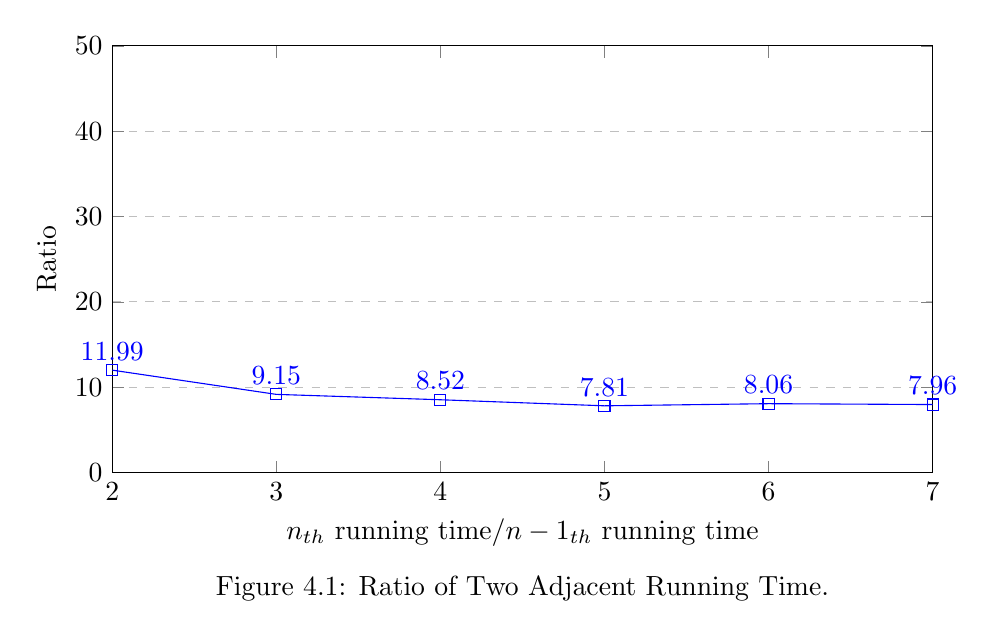
\begin{tikzpicture}
\begin{axis}[
    nodes near coords,%show data.
    width=12cm,height=7cm,
    title style={at={(0.5,0)},anchor=north,yshift=-40},
    title={Figure 4.1: Ratio of Two Adjacent Running Time.},
    xlabel={$n_{th}$ running time/$n-1_{th}$ running time},
    ylabel={Ratio},
    xmin=2, xmax=7,
    ymin=0, ymax=50,
    symbolic x coords={2,3,4,5,6,7},
    xtick=data,
    ytick={0,10,20,30,40,50},
    legend pos=north west,
    ymajorgrids=true,
    grid style=dashed,
]

\addplot[
    color=blue,
    mark=square,
    ]
    coordinates {
    (2,11.99)(3,9.15)(4,8.52)(5,7.81)(6,8.06)(7,7.96)
    };

\end{axis}
\end{tikzpicture}

We can find that the ratio between two adjacent running time is similar, around $10\pm2$.

\section{Conclusion}
In this report, we designed and performed performance experiments for the existing complete program that aims to solve the \emph{Percsort} problem. We designed methods to get results of the memory overhead, CPU overhead, running time and number of loops. We find some interesting results, e.g., the memory overhead and running time have a close coupling, the map size and number of loops have a proportional relationship, and the ratio between two adjacent running time is similar. In the future, we plan to use a higher performance computer to do the above experiments to get a more detailed analysis.


\end{document}
